\documentclass[cs4size,12pt,a4paper]{ctexart}

\usepackage{geometry}%用于设置上下左右页边距
\geometry{top=2.8cm,bottom=2.7cm,left=2.8cm,right=2.8cm}
\usepackage{xeCJK,amsmath,paralist,enumerate,booktabs,multirow,graphicx,subfig,setspace,listings,lastpage,hyperref}
\usepackage{amsthm, amssymb, bm, color, framed, graphicx, hyperref, mathrsfs}
\usepackage{mathrsfs}  
	\setlength{\parindent}{2em}
	\lstset{language=Matlab}%
\usepackage{fancyhdr}
\usepackage{graphicx}
\usepackage{subfloat}
\usepackage{listings}
\usepackage{xcolor}
\usepackage{float}
\usepackage{paralist}
\usepackage{setspace}
\usepackage{titlesec}
\usepackage{enumitem}
\usepackage{hyperref}
\usepackage{multirow}
\usepackage{threeparttable}
\usepackage{autobreak}
\usepackage{multicol}
\usepackage{subfig}
\usepackage{unicode-math}
\usepackage{ltxtable, filecontents}
\usepackage{array}
\usepackage{amsmath}
\usepackage{pifont}
\usepackage{lipsum}
\usepackage{microtype}
\usepackage{wrapfig}
\usepackage{indentfirst}

\setmainfont{Times New Roman}[SmallCapsFont=TeX Gyre Termes:+smcp]

\interfootnotelinepenalty=10000 %强制脚注不换页

\hypersetup{
	colorlinks=true,
	linkcolor=black,
	urlcolor=black
}

\setenumerate{partopsep=0pt,topsep=0pt,itemsep=0pt,leftmargin=2em}
\setitemize{itemsep=0pt,partopsep=0pt,topsep=0pt,leftmargin=2em}

\ctexset{secnumdepth=4,tocdepth=4}
\setlength{\parindent}{2em} %首行缩进两字符
\setstretch{1.5} %英文行距1.45,中文1.5

\setlength{\headsep}{0.5cm} %页眉与正文距离


\setCJKmainfont[BoldFont={FZHei-B01},ItalicFont={FZKai-Z03}]{FZShuSong-Z01} 
\setCJKsansfont[BoldFont={FZHei-B01}]{FZKai-Z03} 
\setCJKmonofont[BoldFont={FZHei-B01}]{FZFangSong-Z02}
\setCJKfamilyfont{zhsong}{FZShuSong-Z01} 
\setCJKfamilyfont{zhhei}{FZHei-B01} 
\setCJKfamilyfont{zhkai}[BoldFont={FZHei-B01}]{FZKai-Z03} 
\setCJKfamilyfont{zhfs}[BoldFont={FZHei-B01}]{FZFangSong-Z02} 
\renewcommand*{\songti}{\CJKfamily{zhsong}} 
\renewcommand*{\heiti}{\CJKfamily{zhhei}} 
\renewcommand*{\kaishu}{\CJKfamily{zhkai}} 
\renewcommand*{\fangsong}{\CJKfamily{zhfs}}

\definecolor{mKeyword}{RGB}{0,0,255}          % bule
\definecolor{mString}{RGB}{160,32,240}        % purple
\definecolor{mComment}{RGB}{34,139,34}        % green
\definecolor{mNumber}{RGB}{128,128,128} 

\lstdefinestyle {njulisting} {
	basewidth = 0.5 em,
	lineskip = 3 pt,
	basicstyle = \small\ttfamily,
	% keywordstyle = \bfseries,
	commentstyle = \itshape\color{gray}, 
	basicstyle=\small\ttfamily,
	keywordstyle={\color{black}},     % sets color for keywords
	stringstyle={\color{black}},       % sets color for strings
	commentstyle={\color{black}},     % sets color for comments
	numberstyle=\tiny\color{black},
	numbers = left,
	captionpos = t,
	breaklines = true,
	xleftmargin = 1.2 em,
	xrightmargin = 0 em,
	frame=tlrb,
	tabsize=4,
	aboveskip = 7 pt, %与代码环境上一行的垂直间距
    belowskip = -2 pt %与代码环境下一行的垂直间距
}

\lstset{
style = njulisting, % 调用上述样式 
flexiblecolumns % 允许调整字符宽度
}

\setlength{\abovedisplayskip}{3pt}
\setlength{\belowdisplayskip}{3pt}

\newcommand \sverb {\;\verb}
\definecolor{shadecolor}{rgb}{0.92,0.92,0.92}

\renewcommand{\arraystretch}{1.23} %表格文字与表格线的距离
\renewcommand{\contentsname}{Content}

\CTEXoptions[today=old] %英文日期

\usepackage{fancyhdr}
\pagestyle{fancy}
%------组名------%
\lhead{\zihao{5} \kaishu 启发式评估报告}
%------文档名------%
\rhead{\zihao{5} \kaishu 刘晓旭、刘承杰、王骁、赵凝晖}
\cfoot{\thepage}
\renewcommand{\headrulewidth}{0.4pt}
\renewcommand{\theenumi}{(\arabic{enumi})}

\titlespacing*{\section}{0pt}{3pt}{3pt}
\titlespacing*{\subsection}{0pt}{2pt}{2pt}
\titlespacing*{\subsubsection}{0pt}{1pt}{1pt}
\titlespacing*{\paragraph}{0pt}{0pt}{0pt}

\CTEXsetup[format={\Large\bfseries}]{section} %设置标题左对齐

\newcommand{\duihao}{\ding{51}\;}
\newcommand{\cuohao}{\ding{55}\;}


\begin{document}
	%---------封面---------%
	\begin{titlepage}
	\newcommand{\HRule}{\rule{\linewidth}{0.5mm}}
    \center 
	
\includegraphics[width=0.6\textwidth]{images/校标,中、英文校名组合.jpg}\\[1cm]  %此处原本宽度为0.7

    \HRule \\[0.5cm]
	{\zihao{0} \textbf{启发式评估报告}}
    \HRule \\[0.5cm]

    \vspace{10pt}
    {\zihao{3}  评估对象:第19组刘洋等所选的以\textbf{软工三}为基础的实践项目}


    \vspace{2cm}

  
    {\zihao{-2} \kaishu 小组成员信息}
    \vspace{-0.3cm}
    {\begin{center}
        \begin{table}[H]\zihao{4}
            \setlength{\tabcolsep}{7mm}
            \centering
            \begin{tabular}{|c|c|c|}
            \hline
            姓名  & 学号        \\ \hline
            刘晓旭 & 201250123  \\ \hline
            刘承杰 & 201250125  \\ \hline
            王骁  & 201250151  \\ \hline
            赵凝晖 & 201250152 \\ \hline
            \end{tabular}
        \end{table}
    \end{center}}

    \vspace{1.5cm}

    % {\zihao{3} In this assignment, I choose \textbf{\textit{Stability vs. Reliability}} and\\[0.3cm] \textbf{\textit{Reusability vs. Portability}}.}

    \vfill

    {\zihao{3}
    \textsc{NanJing University}
    
    \vspace{3pt}
    \textsc{Software Institute}}

    \vspace{0.5cm}
	{\zihao{-3} \today}\\[1cm] 
\end{titlepage}

    %---------目录---------% 
	% \pagenumbering{Roman}
	% \tableofcontents
	% \clearpage

 	%---------正文---------% 
	\pagenumbering{arabic}
	\setcounter{page}{1}

	\section{摘要}
本报告洋细分析了用于评估第19组刘洋等组所选的以其软工三项目为基础的实践项目的启发式评估过程。评估本身是根据雅各布-尼尔森 (lakob Nielse)提供的启发式可用性评估方法进行的。这种方法包括评估人员在尝试完成一项系统任务时,将一组预先确定的可用性原则与应用程序或网站进行比较。

本项目使用了十种启发式方法,重点是其软工三项目的核心功能:进行情绪分析和展示所选APP在一段时间评论的情感热力图和情感趋势图。评估的目的是通过应用这十种启发式方法找出其软工三项目界面的主要缺陷:

\begin{spacing}{1.3}
\vspace{-0.5em}
\begin{multicols}{2}
    \begin{enumerate}[label=\arabic*.]
        \item 系统状态的可见度
        \item 系统和现实世界的吻合
        \item 用户享有控制权和自主权
        \item 一致性和标准化
        \item 避免出错
        \item 依赖识别而非记忆
        \item 使用的灵活性和高效性
        \item 审美感和最小化设计
        \item 帮助用户识别、诊断和恢复错误 
        \item 帮助和文档
    \end{enumerate}
\end{multicols}
\vspace{-0.5em}
\end{spacing}

评估中发现的可用性问题分为7个方面,并根据问题的严重程度和解决的难以程度进行排序。5个最严重和最容易解决的问题分别是:

\begin{enumerate}[label=\arabic*.]
    \item 情感分析结果需要二次展开
    \item 用户手册使用开发语言而不是用户语言
    \item 选择日期错误无法直接在选择界面更改
    \item 显示单词超出范围
    \item 页面使用无意义的初始值
\end{enumerate}

本报告没有详细讨论最后2个可用性问题是:“界面中的默认文本难以阅读”和“系统井不总是为用户提供有关正在执行的任务的足够信息”。这些问题没有详细讨论,因为评估人员把它们归类为肤浅的可用性问题,只有在有额外时间的情况下才应加以解决。
	\section{引言}
本报告介绍了对刘洋组软工三项目的启发式评估过程和结果。报告首先简要介绍了该产品及其目标用户群,然后概述了启发式评估技术的总体情况、本项目的具体目标以及我们在对该应用程序进行演练时使用的启发式评估方法。随后是启发式评估所发现的主要问题的概述,以及与这些具体问题相关的调查结果的详细探讨,这些问题根据其严重程度和对用户体验的影响进行了优先排序。


	\section{产品信息}

\subsection{产品说明}
该项目为软工三大作业项目,其中主要包含两个大部分的内容。第一大部分为情绪分析和解释,通过对情绪分析工具SentiStrength的封装,实现了对用户输入的文本或上传的文件中的内容进行情感分析打分的功能。同时支持用户自定义选择情感分析方式和是否需要解释,同时也支持数十种自定义的文本解析规则,例如是否启用表情识别和自定词典识别等。

第二大部分为根据论文``What parts of your apps are loved by users?"中提到的处理方法对若干APP在应用商店上的评论进行爬取、分析和可视化展示,包括数据热力图和数据趋势图。原论文的背景在于软件开发者经常渴望了解用户喜欢使用他们软件的哪些部分。根据对4000名微软工程师的调查,问题“哪些软件产品的部分(方面) 最受客户使用和/或喜爱?”位列开发者提出的145个问题中的第二位。而用户评论是软件开发者了解用户需求、偏好和抱怨的重要途径。通过分析用户评论,开发者可以评估他们的产品,确定用户的偏好,并改进软件维护和演化任务。该系统通过交互式可视化展示,以便于应用开发者和管理者高效地查看评论的某一时刻的情感侧重点与情感趋势方向,能够高效地总结信息与指定接下来的发展方针。

\subsection{目标人群}
该系统的目标人群是应用开发者、商业分析师和APP爱好者个体。

\begin{figure}[htbp]
	\centering
	\includegraphics[width=\textwidth]{images/首页.png}
	\caption{待评估系统首页}
\end{figure}

	\section{启发式评估技术}

\subsection{方法}
本报告采用启发式评估可用性的方法来总结评估结果。根据知名可用性专家 Jakob
Nielsen 的说法,“启发式评估是指让一小批评估人员检查界面,并判断其是否符合公认的可用性原则(启发式)”(《如何进行启发式评估》)。(如何进行启发式评估。这种方法通常被称为“折扣”可用性技术(Nielsen, 1993, p.160),它允许评估者在一个下午的时间内发现产品或应用程序中可能存在的可用性问题。之后,通过启发式评估所发现的可用性问题可以通过更昂贵、更广泛的用户测试来研究。在进行启发式评估时,评估人员在尝试完成实际的系统任务时,会将一组预先确定的特定可用性原则与产品或网站界面进行比较。评估人员可以单独工作,稍后再汇总评估结果;也可以同时进行评估,每个人专注于几种不同的启发式评估。

\subsection{具体项目目标}
在这个项目中,小组四位成员使用十个启发式方法来发现刘洋组软工三项目界面中的可用性问题。这次评估的重点是项目界面的核心功能:情感评估工具的打分和相关图表的展示。评估人员各自准备了启发式方法的结果,然后四人在联合产品演练中一起评估了其余的启发式方法。较大的问题领域和严重程度是通过小组共识达成的。在编写本报告时没有使用 CUE 启发式评估工具。

\subsection{使用的启发式方法}
使用的十种启发式评估方法及概述如下表。

\begin{spacing}{1.3}
    \centering
    \begin{longtable}{|W{c}{0.8cm}|m{3cm}<{\centering}|m{10.2cm}|}
        \caption{启发式评估方法} \\
        \hline
        \textbf{No.} & \textbf{方法名}        & \multicolumn{1}{c|}{\textbf{描述}}                                                                                              \\ \hline
        1 & 系统状态可见 & 又称为可视性原则,即让用户知道系统在做什么;系统状态有反馈,等待时间要合理 \\ \hline
        2 & 系统与现实世界的匹配 & 又称为环境贴切原则,即使用用户语言,而不是开发者语言;贴近实际生活,而不是学术概念。总之,要使用用户可理解的表现方式;信息展示要自然贴切,逻辑正确,将用户认知成本降到最低 \\ \hline
        3 & 用户可控性/用户自由 & 又称为撤销重做原则,即操作失误可退回;用户经常会误触系统功能,这时就需要一个清晰的“紧急出口”来离开非预期状态,而不是必须拓展一个新窗口 \\ \hline
        4 & 统一和标准 & 又称为一致性原则,即同一事物和同类操作的表示要各处保持一致;不要让用户去考虑不同的单词、场景、动作是否意味着同样的东西;遵循平台规范; \\ \hline
        5 & 防错性 & 又称为防错原则,即比错误提示更友好的是——使用一种谨慎的设计方式,从一开始就防止问题的发生;要么消除容易出错的条件,要么检查这些条件,在用户触发操作时向他们提供确认选项,及早消除误操作  \\ \hline
        6 & 识别胜于回忆 & 又称为易取原则,即让用户辨认或者说识别,是一种比让用户回忆更好的方式;通过将对象 /操作 /选项可视化,减轻用户记忆负担;不应该让用户必须记住对话框的每部分信息,应该在适当的时候,系统自动提供可视化或容易检索的信息提示 \\ \hline
        7 & 使用起来灵活高效 & 又称为灵活高效原则,即通过合理的设计让用户在操作过程中更加灵活、高效;为新手和专家设计定制化的操作方式,例如:为新手提供操作引导,为专家用户提供的快捷操作,这样系统就可以同时满足有经验的用户和没有经验的用户;
        用户可体定制经常使用的操作 \\ \hline
        8 & 美观简洁 & 又称为易读性原则或易扫原则,即减少无关信息,体现简洁美感,网络用户浏览的动作更准确的形容应该是“扫”;对话框不应该包含不相关或不常用的信息;对话框中每增加一个额外的信息单元,都会与相关的信息单元争夺用户注意力,并且会降低信息的相对可见性 \\ \hline
        9 & 帮助用户识别、诊断和从错误中恢复 & 又称为容错原则,即系统出现错误时,要向用户明确的展示错误信息;准确指出问题,积极提供解决方法,协助用户尽快从错误状态中恢复正常 \\ \hline
        10 & 帮助和文档 & 又称为人性化帮助原则,即提供必要的帮助提示与说明文档;无需说明文档就能流畅的使用产品自然是极好的,但是一般文档也很有必要性;文档要易于搜索,关注用户任务,列出具体的执行步骤,并且不要太冗长 \\ \hline
    \end{longtable}
\end{spacing}


\subsection{确定问题的轻重缓急}
为了对启发式评估过程中得出的结果进行有效归类,我们将违反启发式的具体实例归纳为5个问题领域。为了进一步了解每个问题的影响,我们根据可用性原则估算了问题的严重程度以及解决问题的难易程度。影响问题严重性评级的因素包括:问题出现的频率、用户克服问题的难易程度以及问题的持续性——问题是一次就能解决还是每次尝试任务时都会困扰用户。这样就为发现的每个问题得出了双重评级,并以此来确定问题领域的优先次序,以便在本报告中进行介绍。下表定义了所采用的严重性和易修复性评级系统。严重性等级是根据 Jakob Nielsen(可用性问题的严重性等级)定义的。

\begin{spacing}{1.3}
    \centering
    \begin{longtable}{|W{c}{1.2cm}|m{13.5cm}|}
        \caption{严重程度排名} \\
        \hline
        \textbf{评级} & \multicolumn{1}{c|}{\textbf{定义}} \\ \hline
        0 & 违反启发式,但似乎不是可用性问题。 \\ \hline
        1 & 肤浅的可用性问题:用户很 容易解決或极少出现。除非有额外的时间,否则不需要在下一个版本中修复。 \\ \hline
        2 & 小的可用性问题:可能会更频繁地出现或更难克服。下一版本应优先解决这个问题。 \\ \hline
        3 & 主要可用性问题:经常出现且持续存在,或用户可能无法或不知道如何解决问题。需要解決的问题很重要,因此应优先解决。 \\ \hline
        4 & 可用性灾难:严重影响产品的使用,用户无法克服。必须在产品发布前解決这个问题。 \\ \hline
    \end{longtable}
\end{spacing}


\begin{spacing}{1.3}
    \centering
    \begin{longtable}{|W{c}{1.2cm}|m{13.5cm}|}
        \caption{轻松修复排名} \\
        \hline
        \textbf{评级} & \multicolumn{1}{c|}{\textbf{定义}} \\ \hline
        0 & 问题极易解决。一名团队成员即可在下一个版本解决。 \\ \hline
        1 & 问题容易解决。涉及特定界面元素,解决方案明确。 \\ \hline
        2 & 需要花费一定精力才能解决问题。涉及界面的多个方面,或需要开发团队在下次发布前实施更改,或解決方案不明确。 \\ \hline
        3 & 可用性问题很难解决。需要集中精力开发才能在下一个版本发布前完成,涉及界面的多个方面。解决方案可能不会立竿见影,或可能存在争议。 \\ \hline
    \end{longtable}
\end{spacing}
	\section{调查结果概述}
在完成对刘洋组软工三项目的启发式评估后,我们发现了7个违反相关启发式原则的问题领域。下面对这些问题进行了优先排序,最严重和最容易解决的问题列在了前面。在已发现的7个问题领域中,最严重的5个将在本报告中详细讨论。

\begin{spacing}{1.3}
    \centering
    \begin{longtable}{|W{c}{0.7cm}|m{5.5cm}|W{c}{2.5cm}|W{c}{2.5cm}|W{c}{2cm}|}
        \caption{问题领域列表} \\
        \hline
        \textbf{No.} & \multicolumn{1}{c|}{\textbf{问题}}  & \textbf{严重程度排名} & \textbf{易于修复排名} & \textbf{启发式编号}\\ \hline
        1 & 情感分析结果需要二次展开 & 3 & 1 & 7,8 \\ \hline
        2 & 用户手册使用开发语言而不是用户语言 & 3 & 1 & 2,7,10 \\ \hline
        3 & 选择日期错误无法直接在选择界面更改 & 2 & 2 & 3 \\ \hline
        4 & 显示单词超出范围 & 2 & 3 & 4,8  \\ \hline
        5 & 页面使用无意义的初始值 & 2 & 2 & 1,7 \\ \hline
    \end{longtable}
\end{spacing}
	\section{具体问题领域}

\subsection{情感分析结果需要二次展开}

\begin{spacing}{1.3}
    \centering
    \begin{longtable}{|W{c}{0.7cm}|m{5.5cm}|W{c}{2.5cm}|W{c}{2.5cm}|W{c}{2cm}|}
        \hline
        \textbf{No.} & \multicolumn{1}{c|}{\textbf{问题}}  & \textbf{严重程度排名} & \textbf{易于修复排名} & \textbf{启发式编号}\\ \hline
        1 & 情感分析结果需要二次展开 & 3 & 1 & 7,8 \\ \hline
    \end{longtable}
\end{spacing}

\subsubsection{问题}
在情感分析界面,注意到情感分析的打分和解释部分初始时是隐藏起来的,需要用户二次展开。这个问题违反了启发式7和8,这两个启发式建议设计起来应该使整个系统使用起来简单高效,为新手提供操作引导,同时要简洁美观,减少无关信息,取消没必要的操作。

\subsubsection{证据}
在情感分析界面,如图 \ref{问题1} 所示,“打分”和“解释”的具体内容为一个下拉菜单,需要下拉才能展开。

\begin{figure*}[t]
	\centering
	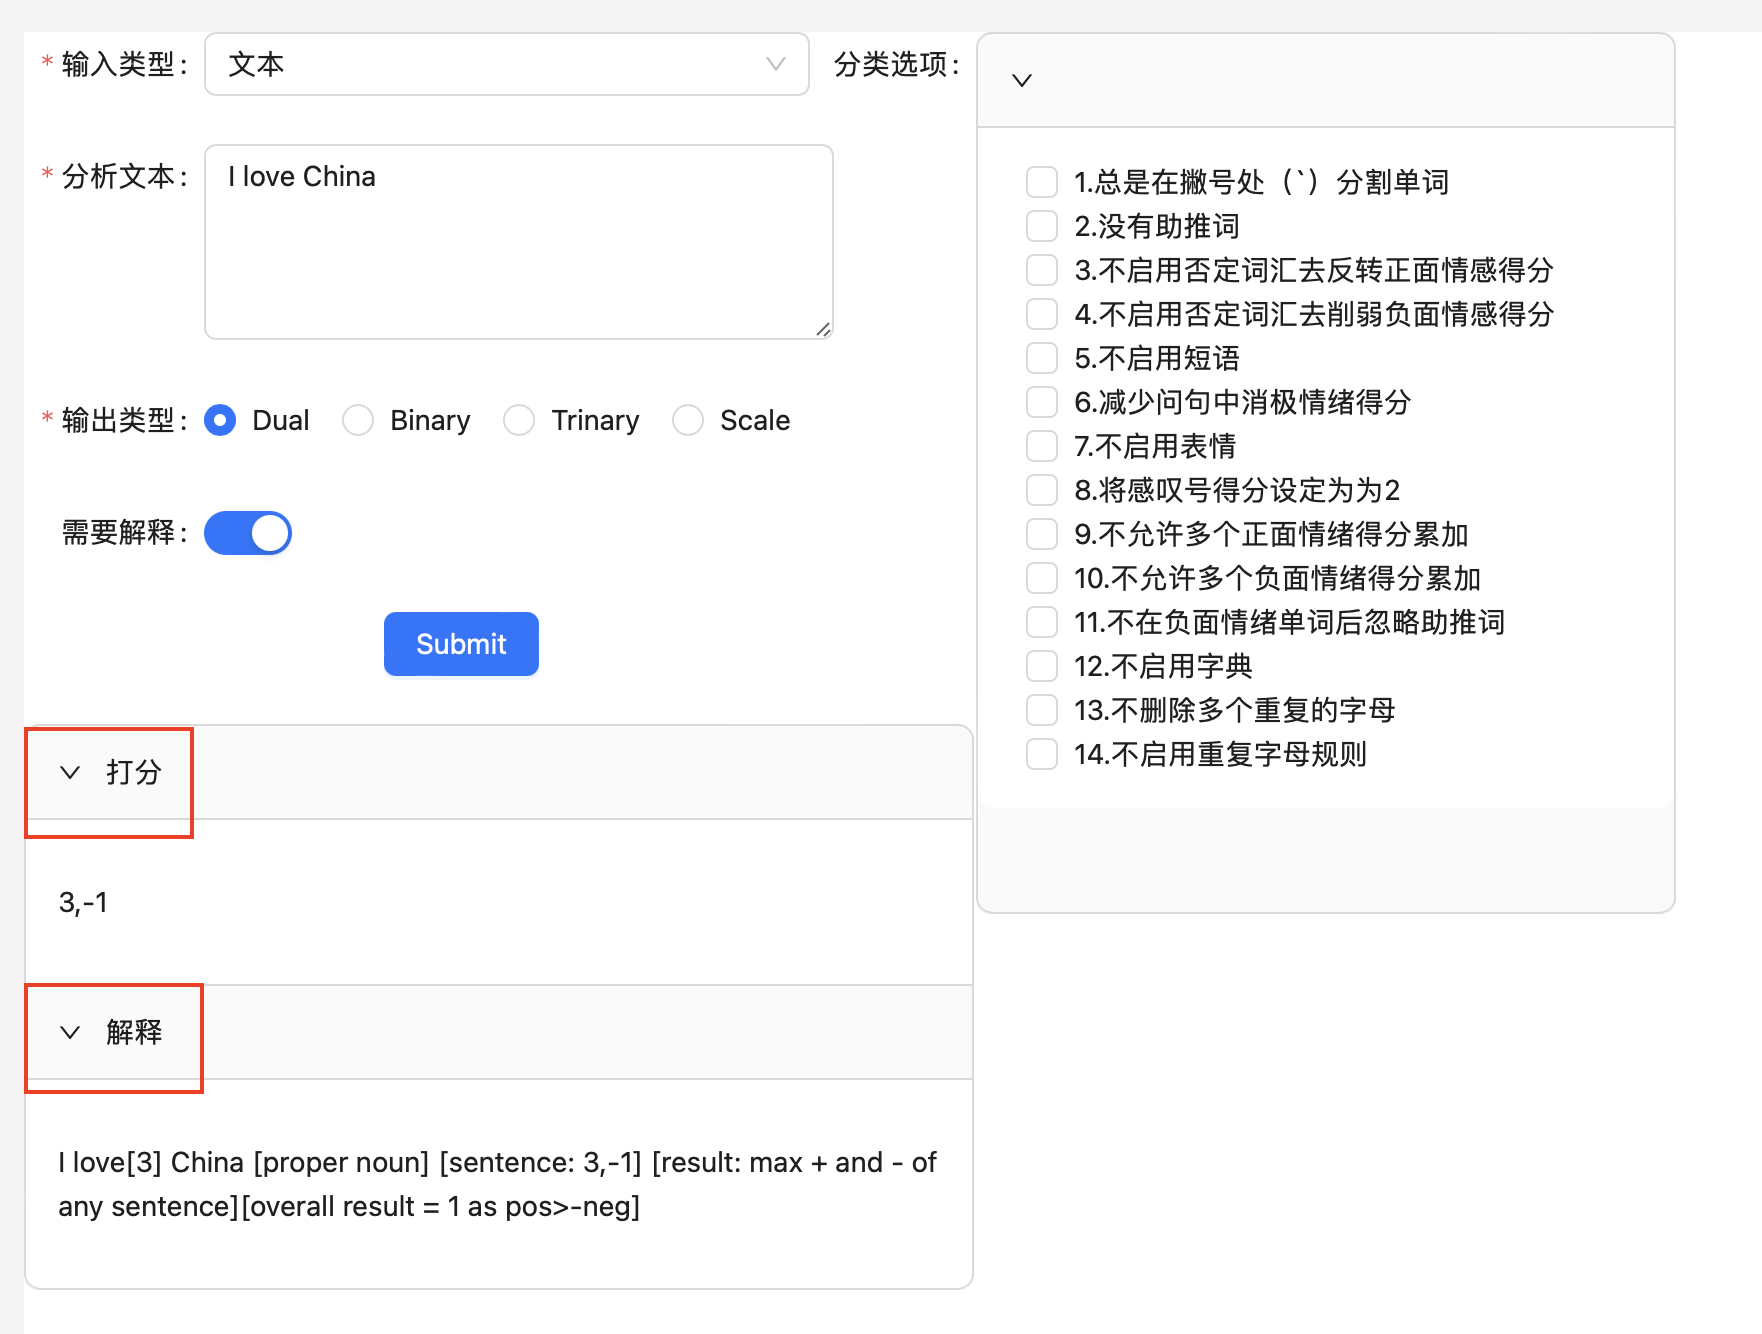
\includegraphics[width=0.98\textwidth]{images/问题1.png}
    \caption{情感分析结果需要二次展开}
    \label{问题1}
\end{figure*}

\subsubsection{建议}
解决这个问题并不难,仅涉及特定界面元素,解决方案明确,只需要设置打分和解释结果默认展开或者干脆取消下拉菜单即可。


\subsection{用户手册使用开发语言而不是用户语言}

\begin{spacing}{1.3}
    \centering
    \begin{longtable}{|W{c}{0.7cm}|m{5.5cm}|W{c}{2.5cm}|W{c}{2.5cm}|W{c}{2cm}|}
        \hline
        \textbf{No.} & \multicolumn{1}{c|}{\textbf{问题}}  & \textbf{严重程度排名} & \textbf{易于修复排名} & \textbf{启发式编号}\\ \hline
        2 & 用户手册使用开发语言而不是用户语言 & 3 & 1 & 2,7,10 \\ \hline
    \end{longtable}
\end{spacing}

\subsubsection{问题}
虽然该系统提供了用户手册,但所用语言过于偏向开发语言,而不是用户语言。这个问题违反了启发式2,7,10。这三个启发式建议系统使用用户语言,贴近实际生活,而不是使用学术概念;同时要对新手提供操作引导,对新手友好;最后提供人性化的帮助,用户帮助和文档要关注用户任务,列出具体的执行步骤,且不要太冗长。这个问题之所以列为可用性问题,是因为其不能通过用户的任何具体操作来解决。

\subsubsection{证据}
在用户手册界面,如图 \ref{问题2} 所示,虽然提供了用户手册,但所用语言对用户并不友好。

\begin{figure}[htbp]
	\centering
	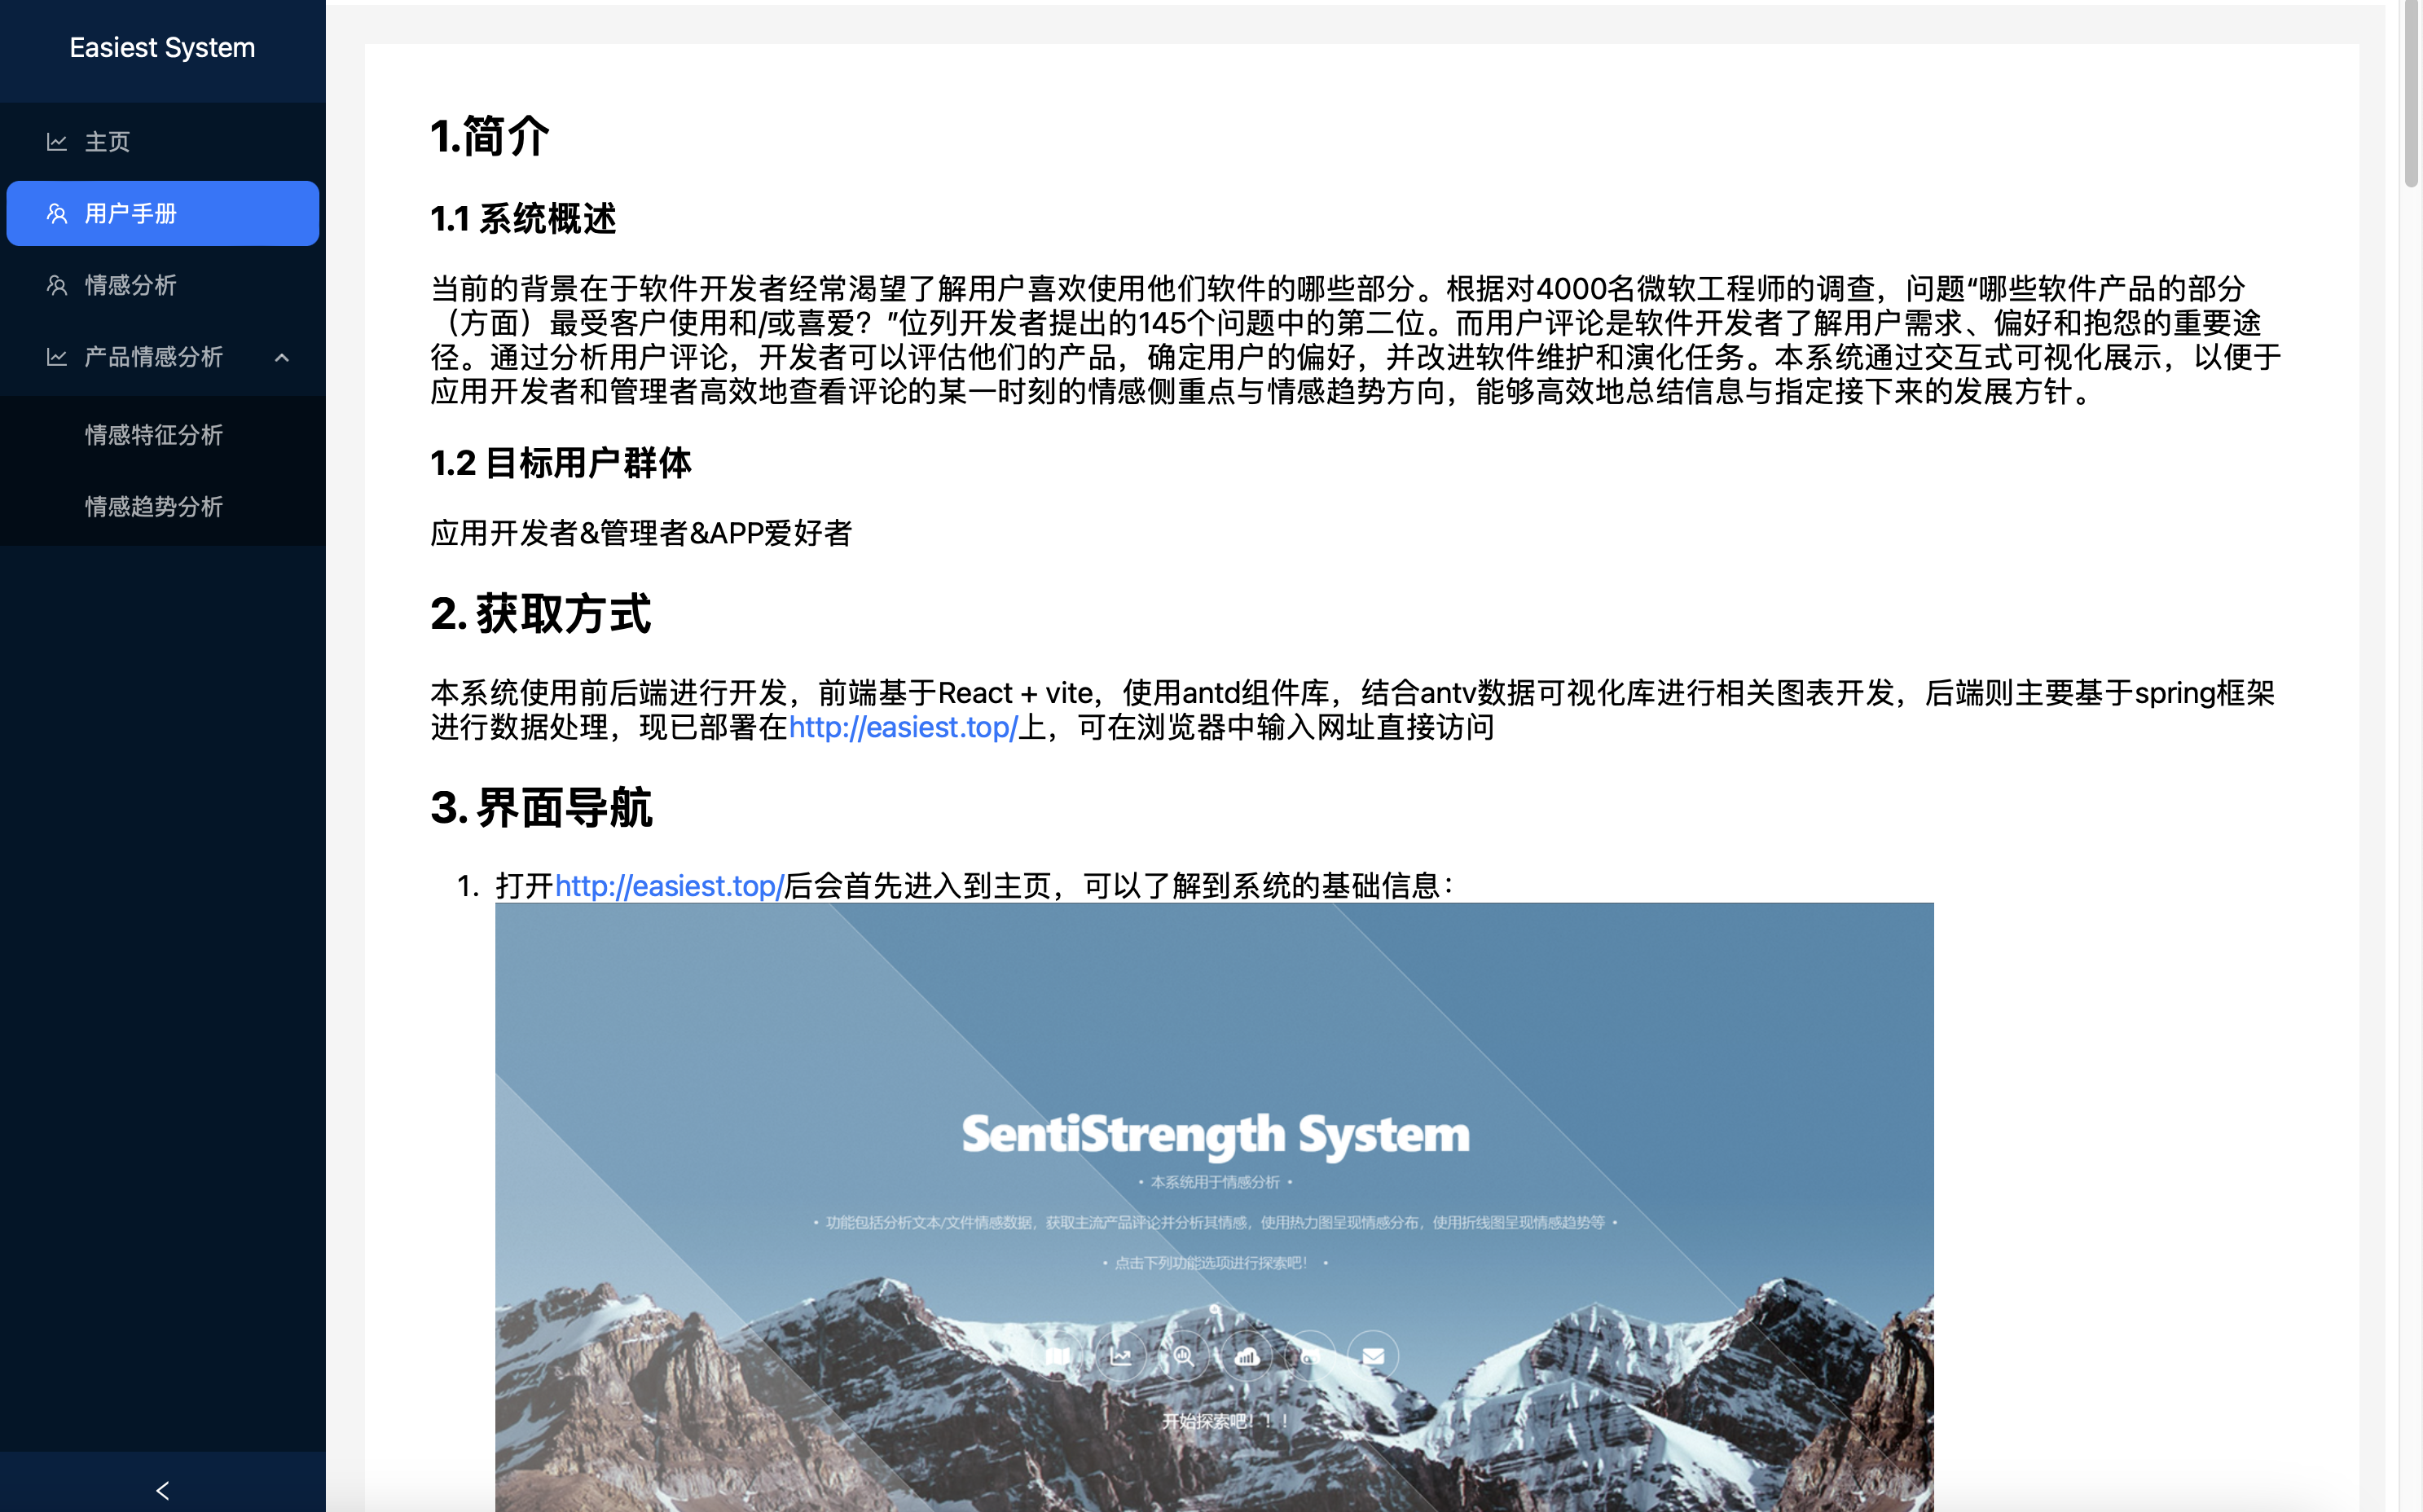
\includegraphics[width=0.98\textwidth]{images/问题2.png}
    \caption{用户手册使用开发语言而不是用户语言}
    \label{问题2}
\end{figure}

\subsubsection{建议}
要解决这个问题,最简单的方式就是对用户手册界面使用用户友好的语言进行重新编写。



\subsection{选择日期错误无法直接在选择界面更改}

\begin{spacing}{1.3}
    \centering
    \begin{longtable}{|W{c}{0.7cm}|m{5.5cm}|W{c}{2.5cm}|W{c}{2.5cm}|W{c}{2cm}|}
        \hline
        \textbf{No.} & \multicolumn{1}{c|}{\textbf{问题}}  & \textbf{严重程度排名} & \textbf{易于修复排名} & \textbf{启发式编号}\\ \hline
        3 & 选择日期错误无法直接在选择界面更改 & 2 & 2 & 3 \\ \hline
    \end{longtable}
\end{spacing}

\subsubsection{问题}
当选择日期错误时,无法直接在选择界面更改,而是需要将两个日期全部选完后,再重新点开日期选择框重新进行选择。这个问题违反了启发式3。这个启发式又称为撤销重做原则,即操作失误可退回:因为用户经常会误触系统功能,这时就需要一个清晰的“紧急出口”来离开非预期状态,而不是必须拓展一个新窗口。这个问题之所以列为可用性问题,是因为其不能通过用户的任何具体操作来解决。

\subsubsection{证据}
如图 \ref{问题3} 所示,当用户选择第一个日期后,前面的日期变得不可选,这种设计能够防止出现用户选择的后一个日期比前一个日期小的问题,但当用户第一个日期选择错误时,将难以进行更改,而是需要随机选择其后面一个日期将整个选择日期的行为完成后,再重新进行日期选择。

\begin{figure}[htp]
	\centering
	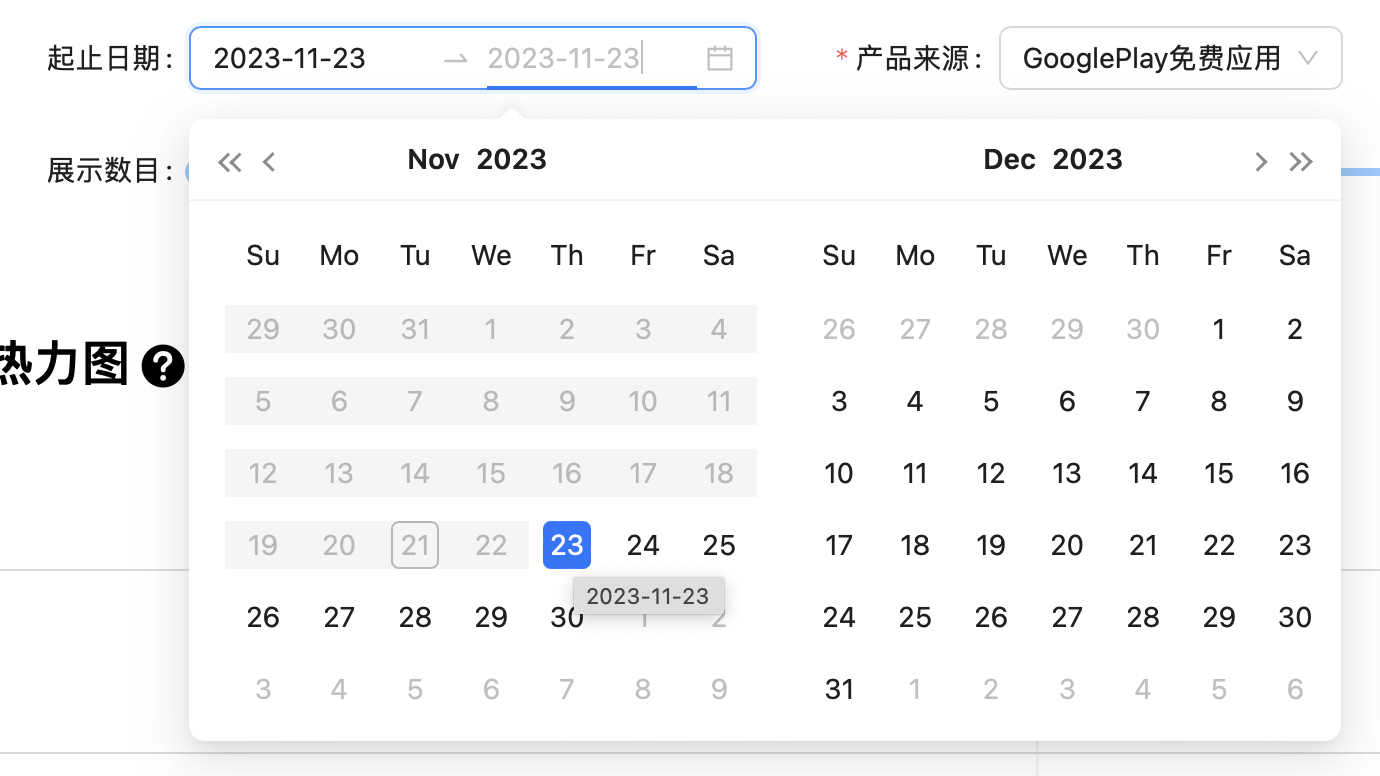
\includegraphics[width=0.7\textwidth]{images/问题3.png}
    \caption{选择日期错误无法直接在选择界面更改}
    \label{问题3}
\end{figure}

\subsubsection{建议}
解决这个问题需要修改日期选择的实现逻辑,当第一个日期已经选定后,不将用户选择这个日期前面的日期的行为视为错误的操作进行限制,而是认为用户是要进行修改,从而将第一个日期更新为所选择的前面日期。

\subsection{显示单词超出范围}

\begin{spacing}{1.3}
    \centering
    \begin{longtable}{|W{c}{0.7cm}|m{5.5cm}|W{c}{2.5cm}|W{c}{2.5cm}|W{c}{2cm}|}
        \hline
        \textbf{No.} & \multicolumn{1}{c|}{\textbf{问题}}  & \textbf{严重程度排名} & \textbf{易于修复排名} & \textbf{启发式编号}\\ \hline
        4 & 显示单词超出范围 & 2 & 3 & 4,8  \\ \hline
    \end{longtable}
\end{spacing}

\subsubsection{问题}
对于特征热力图的展示,原本的设计为每个圆圈表示自动提取的功能组,较大的圆圈表示更受欢迎和喜爱的功能,其中圆圈大小为$\log \mbox{评论数} + \mbox{情感得分}$。这样的设计从数学上看是直观的,但实际显示效果有很大问题。一是圆圈大小看上去都一样,没有什么区别;二是不同单词长度不一样,有的过长单词会显示在圆圈外面。这个问题违反了启发式4和8。

\subsubsection{证据}
如图 \ref{问题4} 所示,圆圈的大小几乎相同,同时过长的单词会超出圆圈的范围。

\begin{figure}[htp]
	\centering
	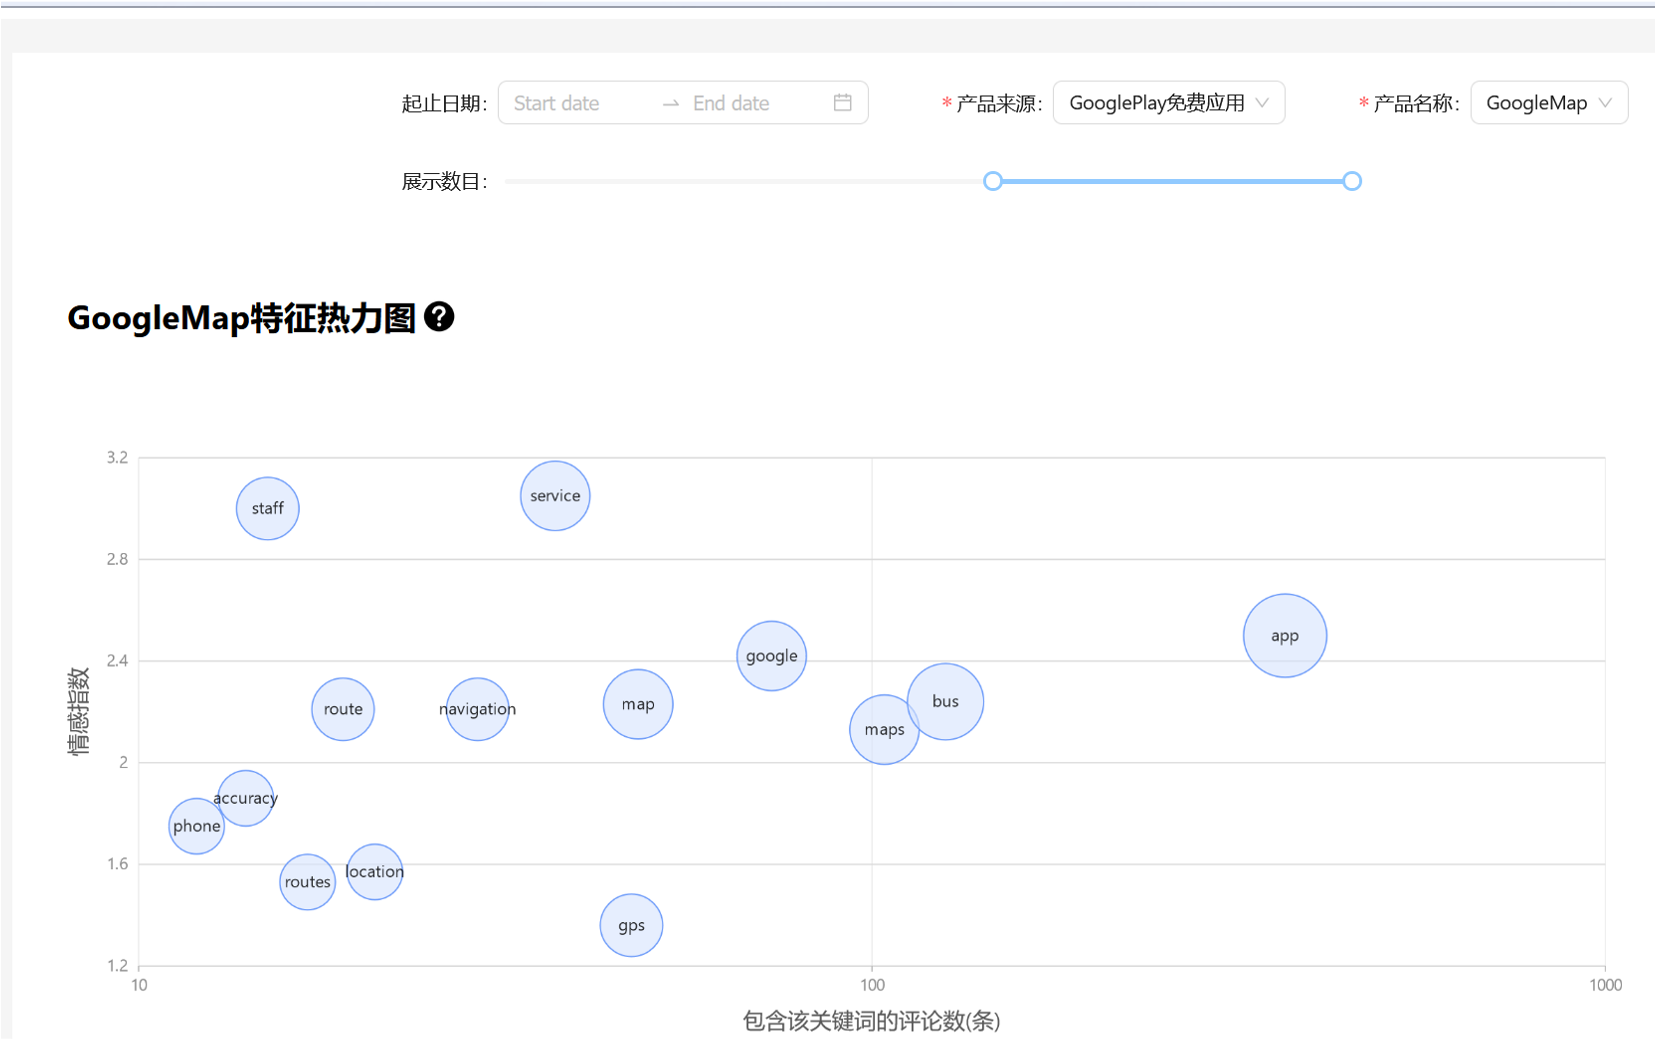
\includegraphics[width=0.98\textwidth]{images/问题4.png}
    \caption{显示单词超出范围}
    \label{问题4}
\end{figure}

\subsubsection{建议}
这个问题并不是很好解决,需要开发团队根据业务需求考虑重新设计圆圈大小的方式,同时根据单词长度进行动态调整字体大小等。


\subsection{页面使用无意义的初始值}

\begin{spacing}{1.3}
    \centering
    \begin{longtable}{|W{c}{0.7cm}|m{5.5cm}|W{c}{2.5cm}|W{c}{2.5cm}|W{c}{2cm}|}
        \hline
        \textbf{No.} & \multicolumn{1}{c|}{\textbf{问题}}  & \textbf{严重程度排名} & \textbf{易于修复排名} & \textbf{启发式编号}\\ \hline
        5 & 页面使用无意义的初始值 & 2 & 2 & 1,7 \\ \hline
    \end{longtable}
\end{spacing}

\subsubsection{问题}
在特征热力图和特征趋势图的初始界面中,也就是用户并没有选择APP和相关时间时,会显示一些无意义的初值,这违反了启发式1和7。无意义的初值的使用让用户并不知道系统在干什么,使系统状态不可见,为用户使用产生困扰。

\subsubsection{证据}
如图 \ref{问题5} 所示,两个界面的初始界面的显示值是无意义的。

\begin{figure}[htbp]
	\setcounter{subfigure}{0}
	\centering
	\subfloat[特征热力图初始界面]{
	    \begin{minipage}[t]{0.99\linewidth}
	    \centering
	    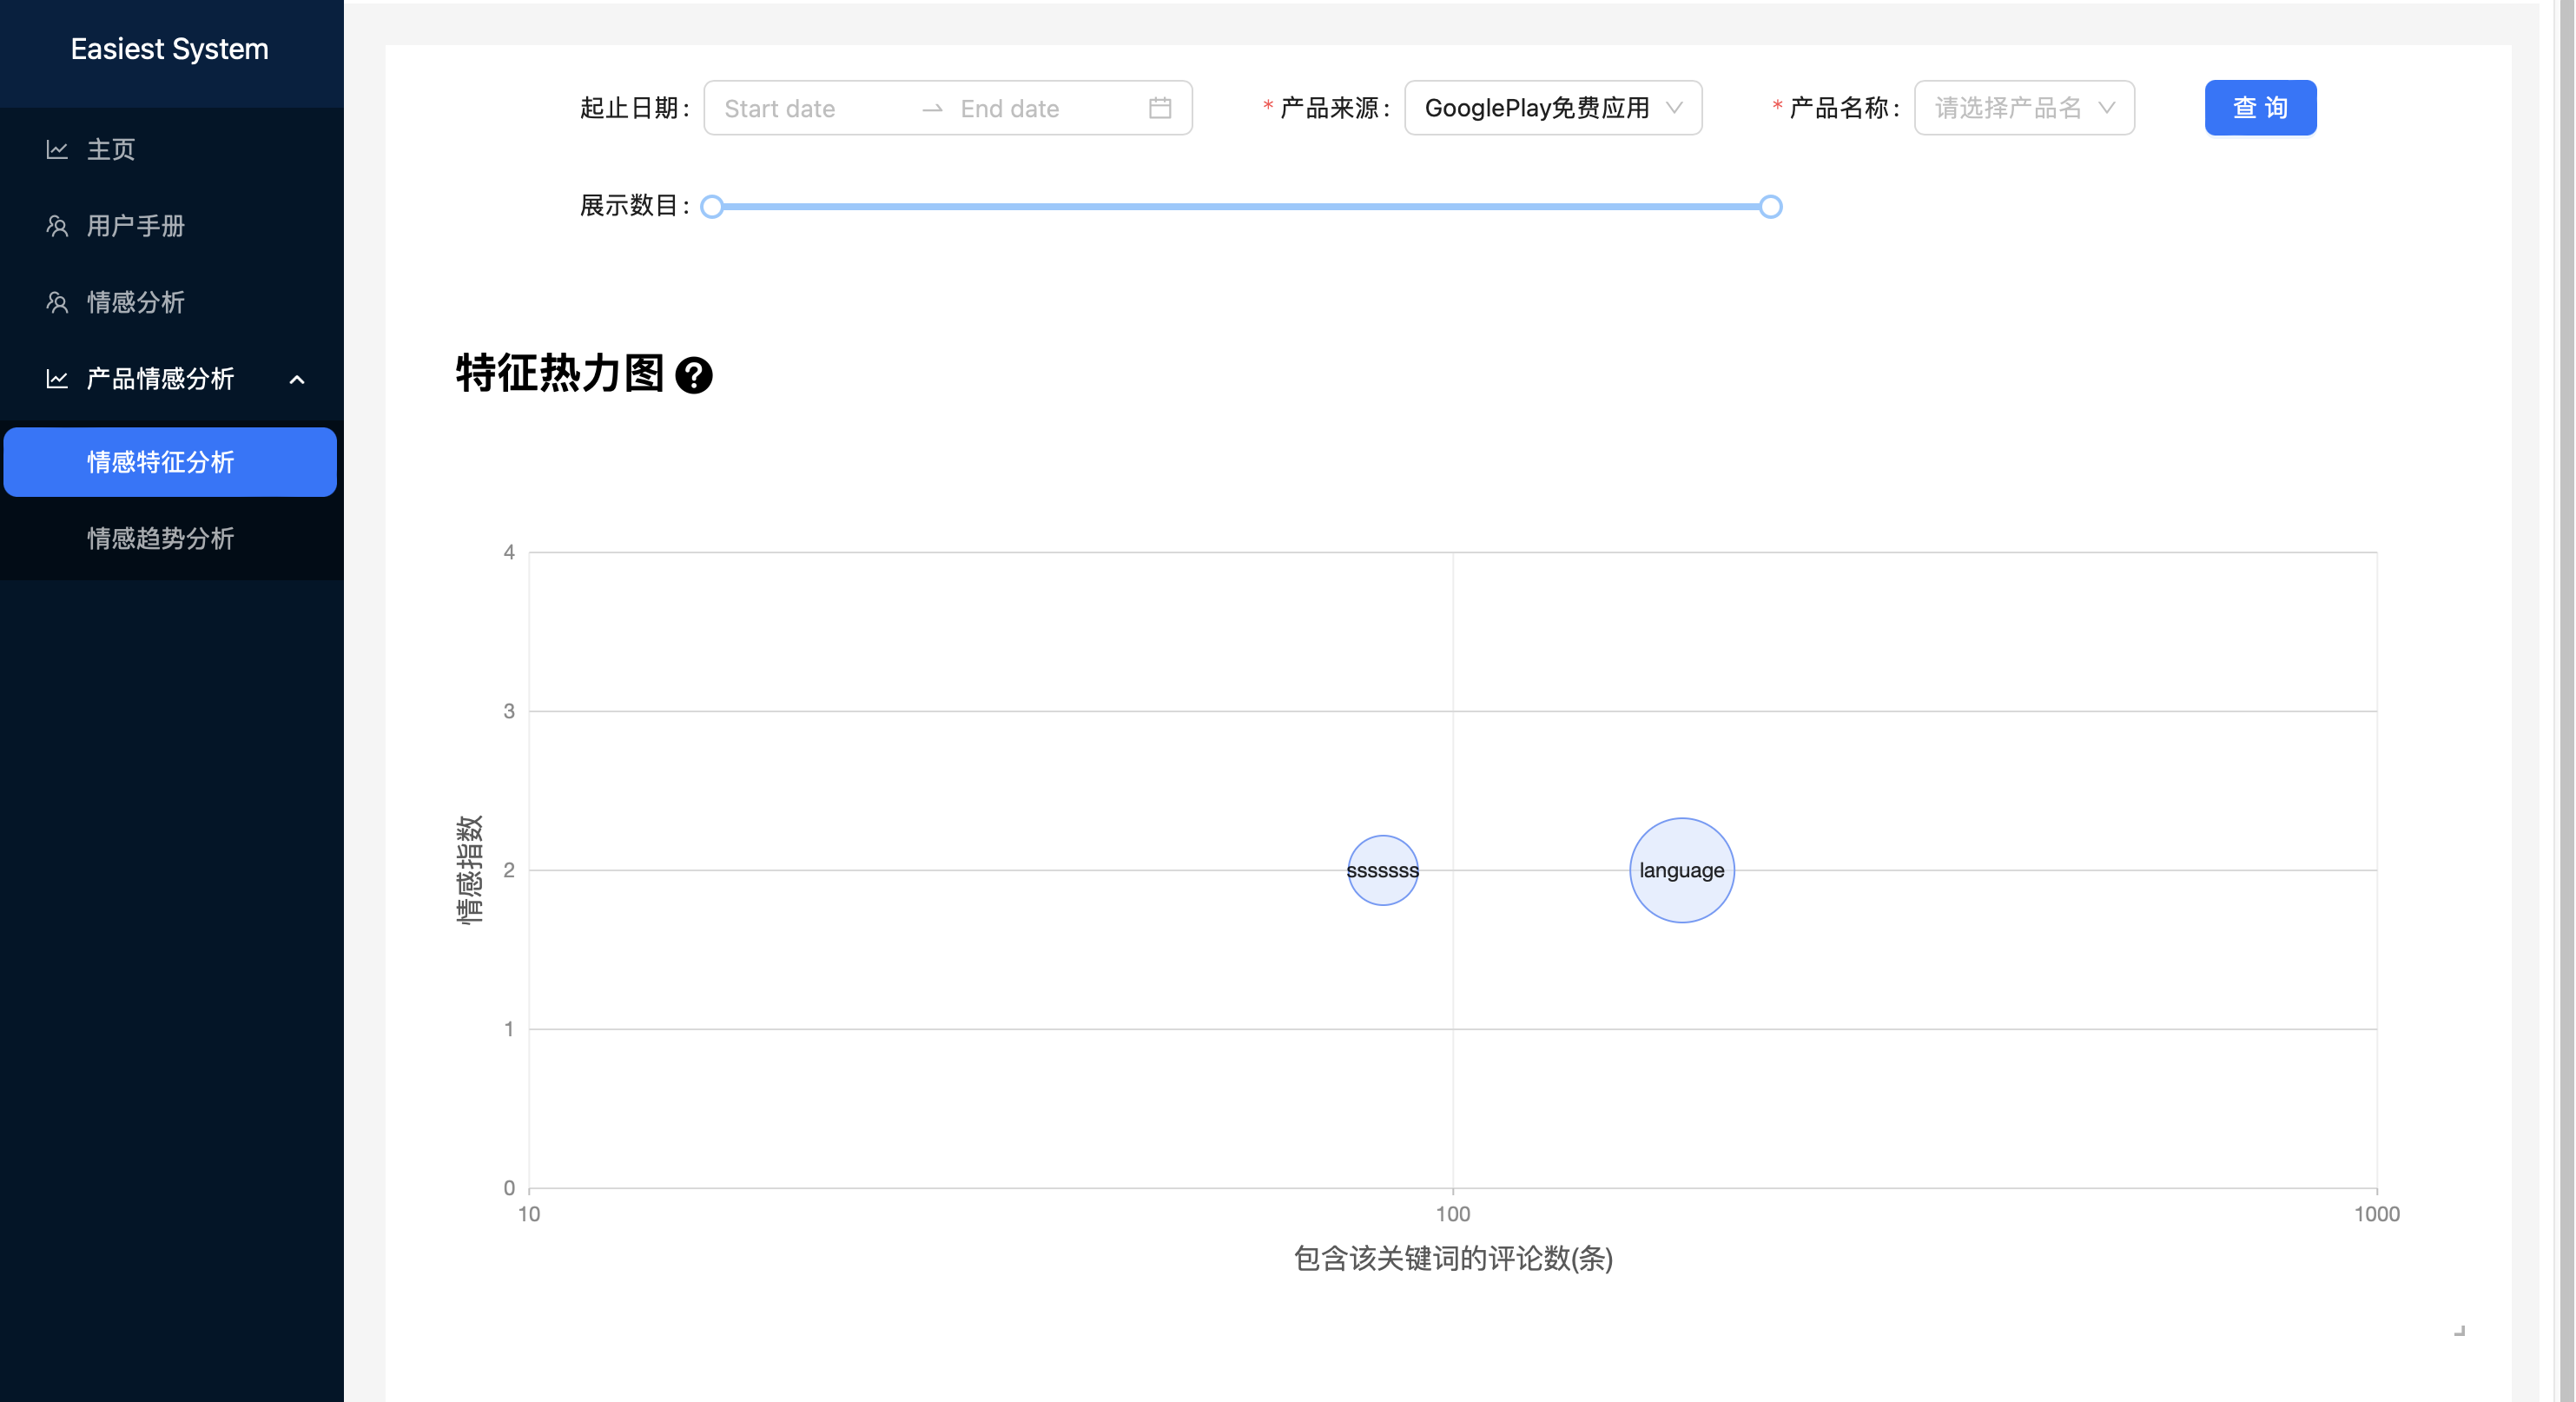
\includegraphics[width=0.98\linewidth]{images/问题5-1.png}
	    \end{minipage}
	}

	\subfloat[特征趋势图初始界面]{
	    \begin{minipage}[t]{0.99\linewidth}
	    \centering
	    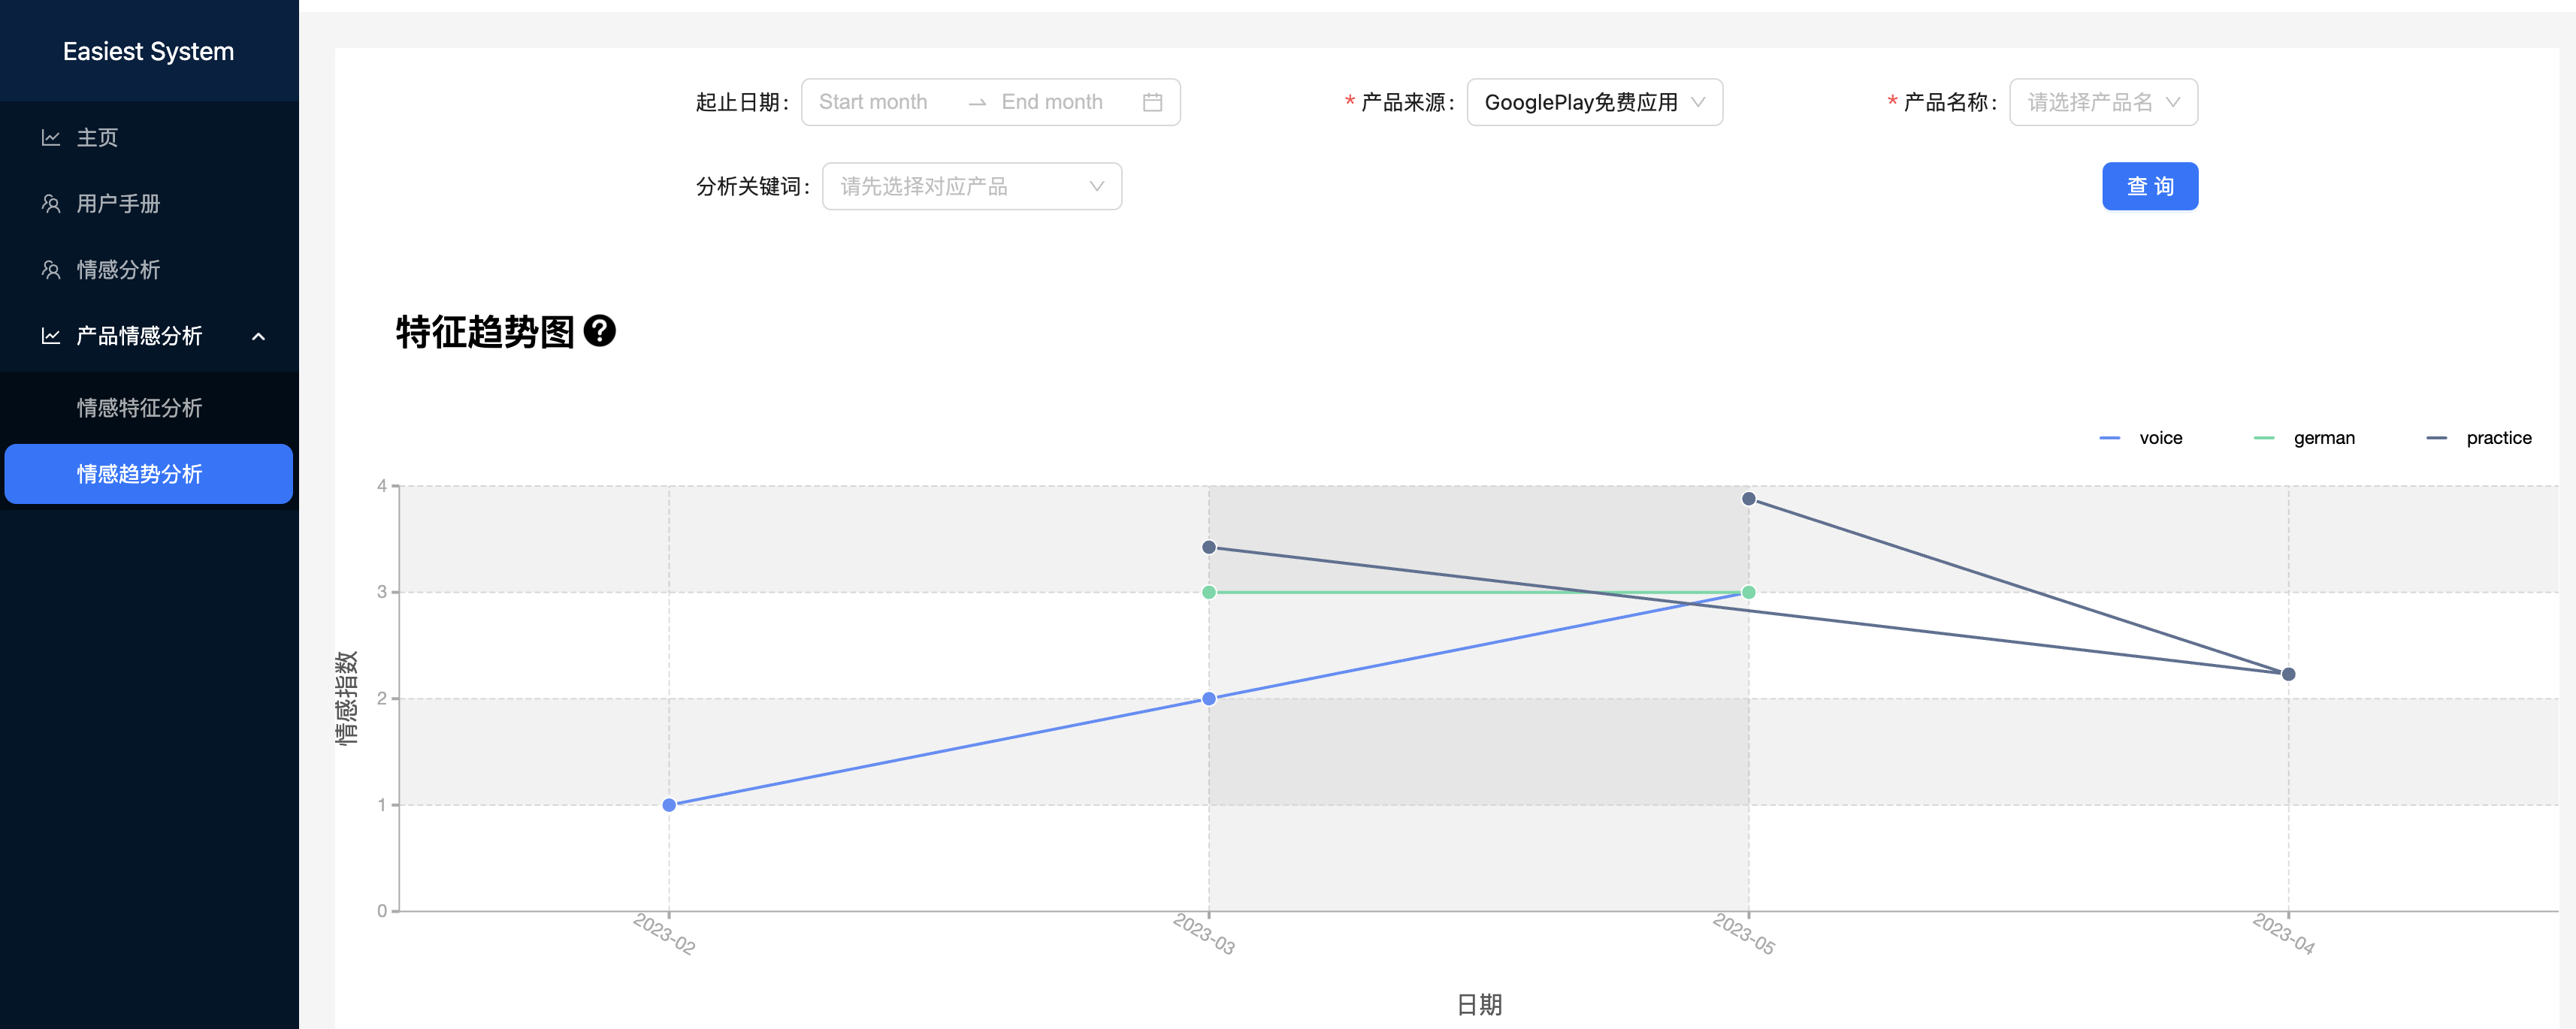
\includegraphics[width=0.98\linewidth]{images/问题5-2.png}
	\end{minipage}
	}
	\centering
	\caption{页面使用无意义的初始值}
    \label{问题5}
\end{figure}

\subsubsection{建议}
这个问题虽然涉及到两个界面,但具体到每个界面的处理还是相对容易的,只需删除初始显示时那些无意义的初值即可,或者在初始显示时对用户进行提示,并换用一些符合现实的初值(而不是这个毫无意义的``sssssss"),让用户理解系统的行为。


\end{document}

% \begin{compactenum}
%     \item 
% \end{compactenum}


% \begin{figure}[H]
%     \vspace{-0.5em}
% 	\centering
% 	\includegraphics[width=0.4\textwidth]{images/}
% 	\caption{}
%     \label{}
%     \vspace{-1em}
% \end{figure}


% \vspace{-0.8em}
% \begin{multicols}{2}
%     \begin{itemize}
%         \item 
%     \end{itemize}
% \end{multicols}
% \vspace{-1em}


% \vspace{-0.5em}
% \begin{spacing}{1.2}
%     \centering
%     \begin{longtable}{|W{c}{2.5cm}|W{c}{3.8cm}|W{c}{4.2cm}|m{4cm}<{\centering}|}
% 		表格内容
% 		表头居中方式  \multicolumn{1}{c|}{表头内容} 
%     \end{longtable}
% 	\end{spacing}
% \vspace{-1em}


% \begin{figure}[htbp]
% 	\setcounter{subfigure}{0}
% 	\centering
% 	\vspace{-0.5em}	
% 	\subfloat[]{
% 	\begin{minipage}[t]{0.33\linewidth}
% 	\centering
% 	\includegraphics[width=0.97\linewidth]{}
% 	\caption{}
%     \label{}
% 	\end{minipage}
% 	}
% 	\subfloat[]{
% 	\begin{minipage}[t]{0.33\linewidth}
% 	\centering
% 	\includegraphics[width=0.97\linewidth]{}
% 	\caption{}
%     \label{}
% 	\end{minipage}
% 	}
% 	\centering
% 	\vspace{-1em}
% 	\caption{}
% \end{figure}


% \begin{wraptable}{r}{6.5cm}
%     \centering
%     \vspace{-1.5em}
%     \begin{tabular}{|c|c|}
%     \hline
%     期望的确定性 & 确定性因子 \\ \hline
%     95\% & 1.960  \\ \hline
%     90\% & 1.645  \\ \hline
%     85\% & 1.281  \\ \hline
%     \end{tabular}
%     \caption*{常见的确定性因子}
%     \vspace{-1.5em}
% \end{wraptable}


% \vspace{-0.5em}
% \begin{shaded}

% \end{shaded}
% \vspace{-1em}
